\documentclass[12pt]{article}

\usepackage{amsmath}
\usepackage{amssymb}
\usepackage{graphicx}
\usepackage{tikz}

\counterwithin*{equation}{section}
\counterwithin*{equation}{subsection}
\addtolength\parskip{\bigskipamount}

\graphicspath{ {./images/} } 

\begin{document}
\section{Partial Derivatives}


Take the derivative of a multivariable function with respect to one variable.
\[
	f_x(x,y) = \lim_{h \to 0} \frac{f(x+h,y) - f(x,y)}{h} = \frac{\partial f}{\partial x}  
\]
\[
	f_y(x,y) = \lim_{h \to 0} \frac{f(x,y+h) - f(x,y)}{h} = \frac{\partial f}{\partial y} 
\]

In general, \(u=f(x_1,x_2,\hdots,x_n)\) 
\[
	\frac{\partial u}{\partial x_i}  = \lim_{h \to 0} \frac{f(x_1,\hdots,x_{i-1},x_i+h,x_{i+1}\hdots,x_n) - f(x_1,\hdots,x_2)}{h}
\]
\underline{Notation} \[
	\frac{\partial u}{\partial x_i} = u'_{x_i}
\]
\underline{Higher Derivatives} \(z=f(x,y)\) 
\[
	(f_x)_x = f_{x x} = f_{11} = \frac{\partial }{\partial x}(\frac{\partial f}{\partial x} ) = \frac{\partial^2f}{(\partial x)^2}  
\]
\[
	(f_y)_y = f_{y y} = f_{22} = \frac{\partial }{\partial y}(\frac{\partial f}{\partial y} ) = \frac{\partial^2f}{(\partial y)^2}  
\]
\[
	(f_x)_y = f_{x y} = f_{12} = \frac{\partial }{\partial x}(\frac{\partial f}{\partial y} ) = \frac{\partial^2f}{\partial x \partial y}  
\]
\[
	(f_y)_x = f_{y x} = f_{21} = \frac{\partial }{\partial y}(\frac{\partial f}{\partial x} ) = \frac{\partial^2f}{\partial y \partial x}  
\]

\subsubsection{Clairaut's Theorem}
Suppose t is defined on a disk \(D\) that contains \((a,b)\) . If \(f_{xy}\) and \(f_{yx}\) are both contoinuous on D, then \[
	f_{xy}(a,b) = f_{yx}(a,b)
\]
\subsubsection{Partial Derivatives Example 1}
Wave Heights\\
\(h=f(v,t)\) \\
Find in notes

\subsubsection{Partial Derivatives Example 2}
\(f(x,y) = x^3 + x^2y^3 - 2y^2\) \\
Find \(f_x(2,1)\) and \(f_y(2,1)\) 

\subsection{Interpretation}
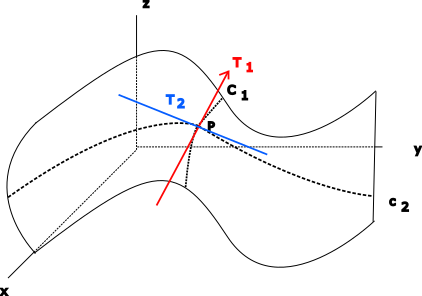
\includegraphics{partialderivativeslopes}\\
\(z=f(x,y)\)\\
\(f(a,b) = C\)\\
\(\rightarrow P(a,b,c)\)
\bigskip\\
Curve \(C_1 =\) where \(y=b\) intersects the surface. \\%
Curve \(C_2 = \) where \(x = a\) intersects the surface.

\(T_1=\) tangent to \(C_1\) at \(P(a,b,c)\rightarrow f_x(a,b) =\) slope of \(T_1\)\\%
\(T_2=\) tangent to \(C_2\) at \(P(a,b,c)\rightarrow f_y(a,b) =\) slope of \(T_2\)

\subsubsection{Partial Derivatives Example 3}
a) Find \(f_x(1,1)\)  and \(f_y(1,1)\) and interpret.\\
\(f(x,y) = 4-x^2-2y^2\) 
\begin{align}
	f_x(x,y) = -2x\\
	f_x(1,1) = -2\\
	f_y(x,y) = -4y\\
	f_y(1,1) = -4
\end{align}

So, the slope at \((1,1,1)\)on the curve of intersection of \(f\) with \(y=1\) is -2.
The slope at \((1,1,1)\) on the curve of intersection of \(f\) with \(x=1\) is -4.

b) Find these tangent lines (TIP: Find curves of intersection)

\subsubsection{Partial Derivatives Example 4}
Find \(\frac{\partial f}{\partial x} \) and \(\frac{\partial f}{\partial y} \) when \(f(x,y) = \sin \frac{y}{1+x}\) 

\subsubsection{Partial Derivatives Example 5}
Find \(z_x\) and \(z_y\) for \(x^4 + y^4 + z^4 + 8xyz = 3\) 

\subsection{Use of PDEs}
\begin{itemize}
	\item Wave Equation
	\item Heat/Diffusion Equation
	\item Maxwell's Equations \(\rightarrow \) E.M
	\item Navier-Stokes \(\rightarrow \) fluid flow
	\item Poisson's Equation \(\rightarrow \) theoretical physics
\end{itemize}

\subsubsection{Partial Derivatives Example 6}
Find the tangent plane to \(z= x^2 + 2y^2\) at point \(P(1,1,3)\) 

\end{document}

